	    \documentclass[a4, 14pts]{seminar}
	    \usepackage[dvips]{pstcol}
	    \usepackage{semcolor}
	    \usepackage{sem-page}
	    \usepackage{slidesec}
	    \input{seminar.bug}
	    \input{seminar.bg2}
	    \usepackage{semhelv}
	    \usepackage{subfigure}
	    \usepackage[latin1]{inputenc}
	    \usepackage[T1]{fontenc}
	    \usepackage{times}
	    \usepackage{longtable,array,enumerate}


	    \usepackage{multicol}

	    \usepackage[intlimits,sumlimits,namelimits]{amsmath}
	    \usepackage{amssymb}
	    \usepackage[mathscr]{eucal}
	    \usepackage{mathrsfs}
	    \usepackage{amsthm}
	    \usepackage{amsfonts}
	    \usepackage{amsmath}

	    \usepackage[dvips]{graphicx}
	    \usepackage{epsf}
	    \usepackage{epsfig}
	    \usepackage{fancyhdr}
	    \usepackage{layout}

	    \usepackage[french]{babel}
	    \usepackage[T1]{fontenc}
	    \usepackage[latin1]{inputenc}

	    \usepackage{url}
	    \usepackage{xspace}

	    \newtheorem{corollary}{Corollaire}[section]
	    \newtheorem{definition}[corollary]{D\'{e}finition}
	    \newtheorem{equations}[corollary]{Equations}
	    \newtheorem{example}[corollary]{Exemple}
	    \newtheorem{lemma}[corollary]{Lemme}
	    \newtheorem{proposition}[corollary]{Proposition}
	    \newtheorem{remark}[corollary]{Remarque}
	    \newtheorem{theorem}[corollary]{Th\'{e}or\`{e}me}
	    %%% The above 7 commands are used in the following way:
	    %%% The definition environment, for example, is created by
	    %%% \begin{definition}\label{xxx}. . .\end{definition}
	    \newcommand{\mylabel}[1]{\label{#1}
			\ifx\undefined\stillediting
			\else \fbox{$#1$}\fi }
	    \newcommand{\BE}{\begin{equation}}
	    \newcommand{\BEQ}[1]{\BE\mylabel{#1}}
	    \newcommand{\EEQ}{\end{equation}}
	    \newcommand{\rfb}[1]{\mbox{\rm
	      (\ref{#1})}\ifx\undefined\stillediting\else:\fbox{$#1$}\fi}
	    \newcommand{\half}   {{\frac{1}{2}}}
	    \newenvironment{matr}[1]{\left[ \begin{array}{#1}}{\end{array}
				    \right]}
	    %
	    \newfont{\Blackboard}{msbm10 scaled 1200}
	    \newcommand{\bl}[1]{\mbox{\Blackboard #1}}
	    \newfont{\roma}{cmr10 scaled 1200}

	    \newcommand{\propp}{{\hskip -2.2mm{\bf .}\hskip 3mm}}

	    \newcommand{\ovra}{\overrightarrow}
	    % fin des commandes de Marius

	    \fancyhf{}
	    \renewcommand\headrulewidth{0.2mm}
	    \renewcommand\footrulewidth{0.2mm}


	    \newcommand{\R}{\mathbb{R}}
	    \newcommand{\C}{\mathbb{C}}
	    \newcommand{\N}{\mathbb{N}}
	    \newcommand{\Z}{\mathbb{Z}}

	    \newcommand{\ROT}{{\text{Rot}}}
	    \newcommand{\Rot}{\vec{\text{Rot}}}
	    \newcommand{\rot}{\vec{\text{rot}}}

	    \newcommand{\dsp}{\displaystyle}

	    \newcommand\eads{\textsf{}\xspace}
	    \newcommand\eadsccr{\textsf{}\xspace}

	    \fancyhead[L]{\theslideheading}
	    \fancyhead[R]{\textcolor{blue}{\eadsccr \thepage }}
	    \fancyfoot[R]{\textcolor{blue}{}}
	    \fancyfoot[L]{\textcolor{blue}{ISWAG Deauville, 3 June 2015 }}
	    \renewcommand\headwidth{\textwidth}
	    \autoslidemarginstrue

	    \newslideframe{%
	      myscshadow}[\SemcolorFrameOps
	      \psset{shadowcolor=green}]{\psshadowbox{#1}}
	    \newcommand{\ud}{\mathrm{d}}

	    \newcommand{\ds}{\displaystyle}
	    \slideframe{myscshadow}
	    \setlength\slideframewidth{.5pt}
	    \setlength\footskip{1cm}
	    \setlength\headsep{1cm}

	    %\renewcommand\makeslideheading[1]{\par
	    %   \framebox{\theslidesection. #1}\par
	    %}
	    %\renewcommand\makeslidesubheading[1]{\par
	    %   \leavevmode\hspace*{1cm}%
	    %   \alph{slidesubsection}. #1\par
	    %}

	    \definecolor{Pink}{rgb}{1.,0.,0.2}
	    \definecolor{Mygreen}{rgb}{0.3,0.7,0.6}

	    \renewcommand\makeslideheading[1]{\par
	      \fcolorbox{black}{Mygreen}{\color{yellow}\theslidesection. #1}\par
	    }
	    \renewcommand\makeslidesubheading[1]{\par
	      \leavevmode\hspace*{1cm}%
	      \textcolor{Mygreen}{\alph{slidesubsection}. #1}\par
	    }

	    \makeatletter
	    \renewcommand\slide@contents{\par
	      \begin{center}
		    \Large \bfseries\textcolor{blue}{Plan}
	      \end{center}
	      \def\l@slide##1##2##3{%
		\@undottedtocline{1}{1.5em}{2.3em}{\slidenumberline{##1.}{##2}}{}}%
	      \def\l@subslide##1##2##3{%
		\@undottedtocline{1}{1.5em}{3.3em}{\slidenumberline{\@alph{##1})}{##2}}{}}%
	      \@startlos
	    }
	    \makeatother

	    \slideframe{none}
	    %\XgrDefinitFormat{*}{line=0,mark=0,ll=1}
	    %\XgrDefinitFormat{pr}{}
	    %\XgrDefinitFormat{ks}{line=-1,mark=8,ll=0.4}
	    \begin{document}
	    \slidepagestyle{fancy}
	    %%%%%%%%%%%%%%%%%%%%%%%%%%%%%%%%%%%%%%%%%%%%%%%%%%%%%%%%%%%%%%%%%%%%%%%%%%%
	    \begin{slide}
	    \thispagestyle{plain}
	    \begin{center}
	    \textcolor{blue}{\huge Internal mesh optimization}\\
	    \textcolor{blue}{\huge Semantic linking and siloing}\\
	    \textcolor{blue}{\huge Big data}\\
	    \vspace{0.25 cm}
	    \textbf{DUPREY Stefan}\\
	    \small{\textbf{Cdiscount}\\ 

	    }
	    %\eadsccr
	    \end{center}
	    \end{slide}
	    %%%%%%%%%%%%%%%%%%%%%%%%%%%%%%%%%%%%%%%%%%%%%%%%%%%%%%%%%%%%%%%%%%%%%%%%%%
	    %%%%%%%%%%%%%%%%%%%%%%%%%%%%%%%%%%%%%%%%%%%%%%%%%%%%%%%%%%%%%%%%%%%%%%%%%%%
	    {\small{
	    \begin{slide}
	    \slidecontents
	    \renewcommand\theslideheading{Plan}
	    \end{slide}
%	    \begin{slide}
%	    \slideheading{Introduction}
%	    \textbf{\textcolor{blue}{\large Objective : give you an overview of the meshing optimization done at Cdiscount, the first french e-commerce web site }}
%	    \small{
%	    \newline $\bullet$ Heuristic based optimization algorithm to push specific products 
%	    \newline $\bullet$ An e-commerce pitch
%	    \newline $\bullet$ Semantic similarity and constraining for shrinking our universe
%	    \newline $\bullet$ Big data implementation
%	    }
%	    \end{slide}
	    \begin{slide}
	    \slideheading{Heuristic}
	    \textbf{\textcolor{blue}{\large Some notations}}\newline
	    Let $N\in\mathbb{N}$ be the number of nodes in our mesh.
	    \newline
	    Let $\left(X_i\right)_{i \in \left\{1,...,N\right\}}$ be the vertices (URLs) of our oriented graph.
	    \newline
	    Let $\left(G_{ij}\right)  \in \left\{0,1\right\}^{N\times N}$ be the adjacency matrix of our oriented graph.
	    \newline
	    Let here define f, a given data per URL, which gives a potentiality metrics for our vertices.
	    \begin{equation}
	    \begin{array}{ccccc}
	    f & : & \left(X_i\right)_{i \in \left\{1,...,N\right\}} & \to & \mathbb{R}^{+} \\
	    & & x & \mapsto & f(x) \\
	    \end{array}
	    \end{equation}
	     \begin{equation}
	    f(X_i) = PR_{ext}(X_i) +  \epsilon \left(X_i\right)
	    \end{equation}
	    \end{slide}
	    \begin{slide}
	    \textbf{\textcolor{blue}{\large In-rank}}\newline      
	    We restrain the universe to our site where we compute the standard page-rank.
	    \newline
	    Initialization :
	    \begin{equation}
	    \forall u \ PR\left(u\right)=\frac{1}{N}
	    \end{equation} 
	    Iterative computation :
	    \begin{equation}
	    PR\left(u\right)= \frac{\left(1-c\right)}{N} + c \times \sum_{v \rightarrow u}\frac{PR\left(v\right)}{card\left(\left\{v\rightarrow u\right\}\right)}
	    \end{equation}
	    \end{slide}
	    \begin{slide}
	    \textbf{\textcolor{blue}{\large Our heuristic}}\newline 
	    We want here to optimize the adequacy of our mesh $\left(X_i\right)$ to our potentiality vector $f$.
	    We here postulate the following heuristic to assess the relevance of a mesh :
	    \begin{equation}
	    \max_{\left(G_{ij}\right)  \in \left\{0,1\right\}^{N\times N}}\left\{ \sum^{N}_{i=1} trafic\left(X_i\right)\times pageRank(X_i)\right\}
	    \end{equation} 
	    \end{slide}

	    \begin{slide}
	    \slideheading{Metaheuristics}    
	    \textbf{\textcolor{blue}{\large Exhaustive brute force doesn't work}}\newline
	    For a $N=10^6$ millions URLs web site, we have $2^{N^{2}}$ with a 2048 bits mantissa, 256 bits exponent 
	    \newline
	    \scriptsize{
	    $2^{{10^6}^2}=$
	    \\ \newline 9.5762442314927432848050594956989483747127095675192905698213128517073583274396016675898
	    \\ \newline 714705184143146468453752442806484690561169975498415015777492655947375270159476651418975
	    \\ \newline 300707658547568802353384879419803574730952480197774380552040662758127609571333683703207
	    \\ \newline 910070247048194459504686986124786492353387550318495241621572271925127288273993787778380
	    \\ \newline 450774809611395810191417363401889038757182279484019203870177413318113073911418463615759
	    \\ \newline 647977538478560166958988721048687854280187283661925937530017243461145905573802314471888
	    \\ \newline 491758757162677684017424597014433418179115289463552630751896559312213624470617453325056
	    \\ \newline 5836008e+301029995663
	    }
	    \end{slide}
	    \begin{slide}
	    \textbf{\textcolor{blue}{\large Picturing our smallest store : jewelery}}\newline  
	    \begin{center}
	    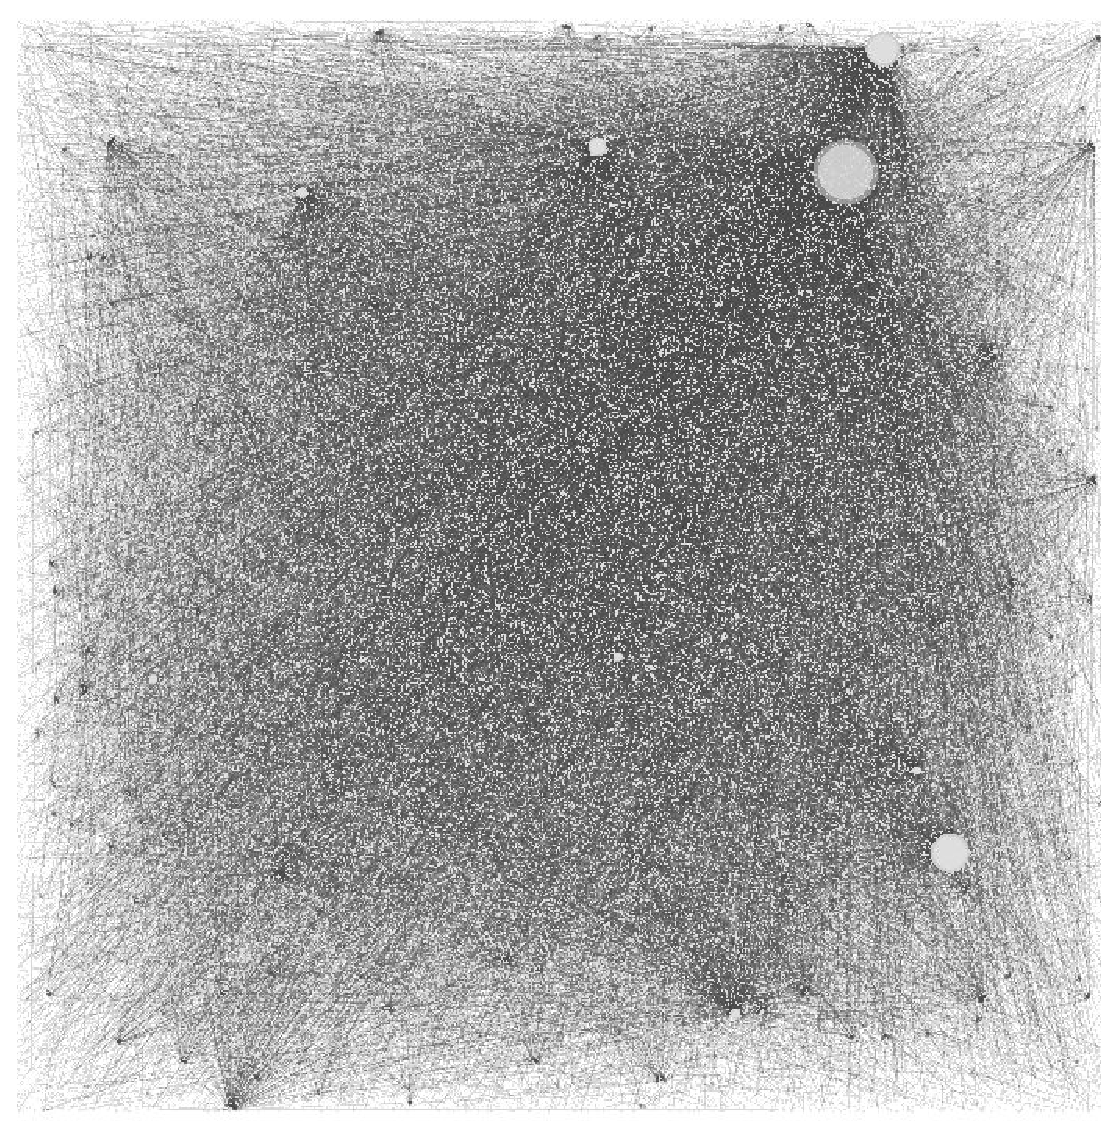
\epsfig{file=page_rank.eps,height=6.5cm,width=8.cm}
	    \end{center}
	    \end{slide}
	    \begin{slide}
	    \textbf{\textcolor{blue}{\large Metaheuristics}}\newline
	    We here have to maximize over all possible graphs. 
	    We have to find a clever global optimization methodology : metaheuristics such as global search, multistart, particle swarm, simulated annealing or genetic algorithm are all good candidates.
	    \newline 
	    \textbf{\textcolor{black}{\normalsize What is a genetic algorithm}}
	    \scriptsize{
	    \newline $\bullet$ Genetic algorithm mimics evolutionary biology to find approximate solutions to optimization problems 
	    \newline $\bullet$ Start with an initial generation of candidate solutions that are tested against the objecive function (fitness of the individual)
	    \newline $\bullet$ Subsequent generations evolve from the first through selection, crossover and mutation
	    \newline $\bullet$ The individual that best minimizes the given objective is returned as the ideal solution
	    }
	    \newline \textbf{\textcolor{black}{\normalsize Why a genetic algorithm}}
	    \scriptsize{
	    \newline $\bullet$ Lots of local minima to avoid
	    \newline $\bullet$ Non continuous universe, constraints and objective
	    \newline $\bullet$ Problem with noise and non-smooth data
	    }
	    \end{slide}
	    \begin{slide}
	    \textbf{\textcolor{blue}{\large Cleverly evolving through our universe}}\newline
	      \begin{center}
	      \textbf{\large Child spawning from 2 parents crossover}
	      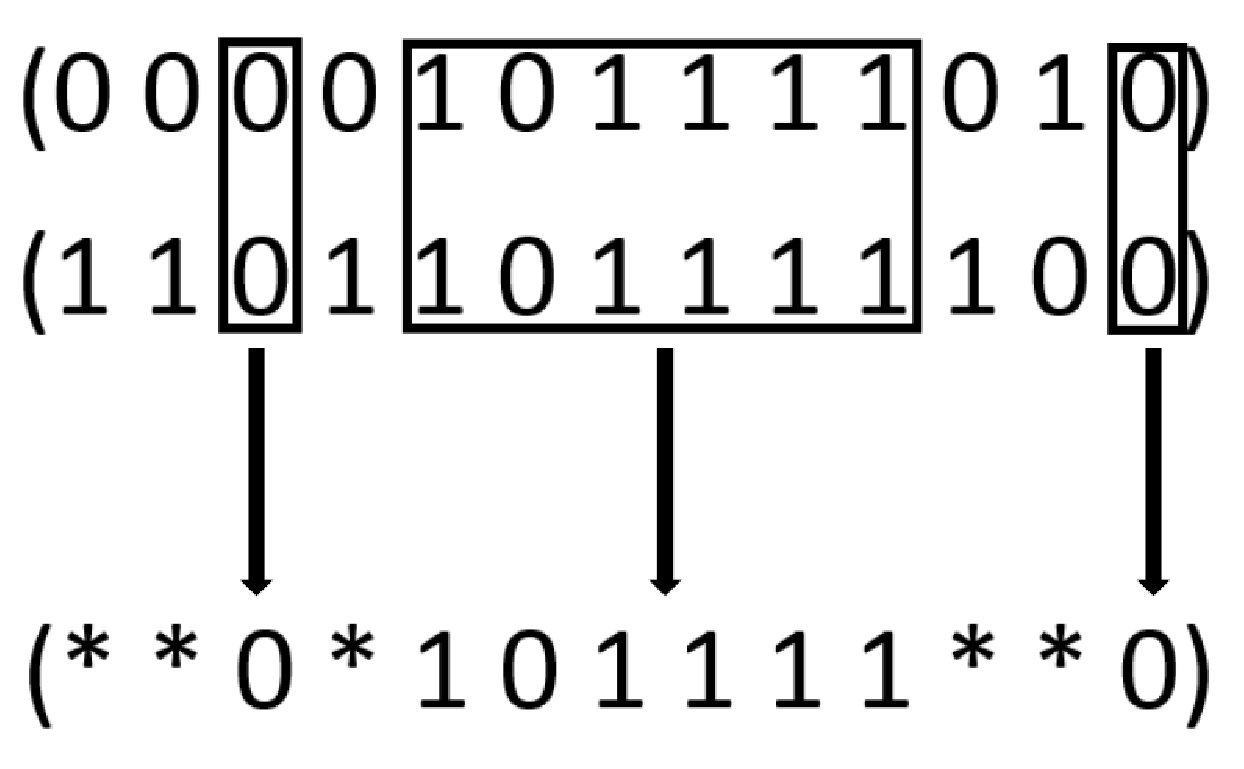
\epsfig{file=crossover.eps,height=2cm,width=4cm}
	      \end{center}
	      \begin{center}
	      \textbf{\large Mutation of an individual}
	      \end{center}
	      \begin{center}
	      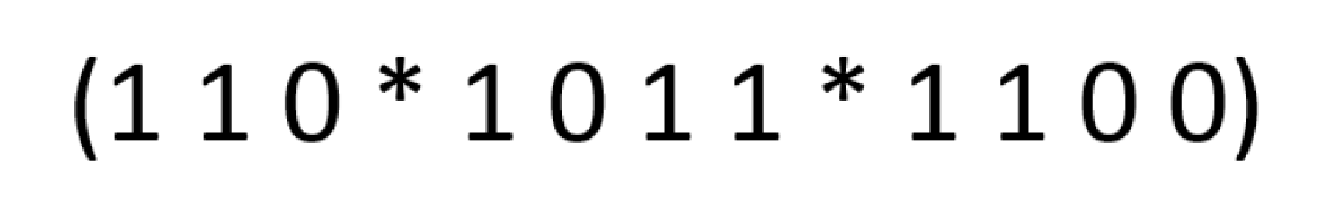
\epsfig{file=mutation.eps,height=0.4cm,width=4cm}
	      \end{center}
	    \end{slide}
	    \begin{slide}
	    \slideheading{Shrinking our universe with siloing and semantic similarity}
	      \textbf{\textcolor{blue}{\large Siloing and links categorizing}}\newline
	      \begin{center}
	      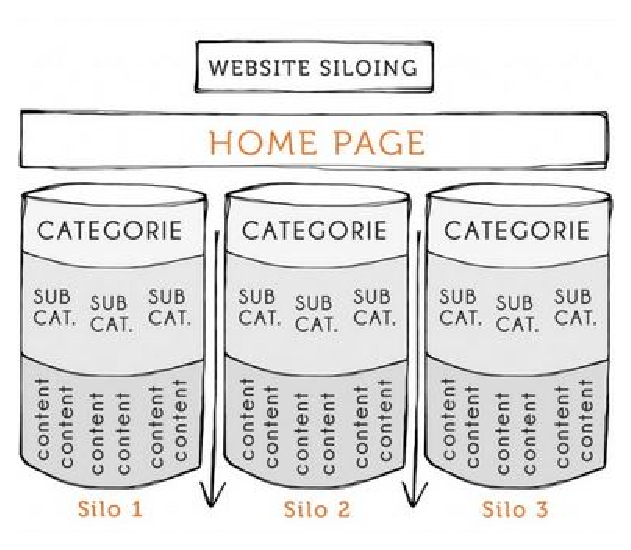
\epsfig{file=website_siloing.eps,height=4cm,width=6cm}
	      \end{center}
	    \begin{center}
	      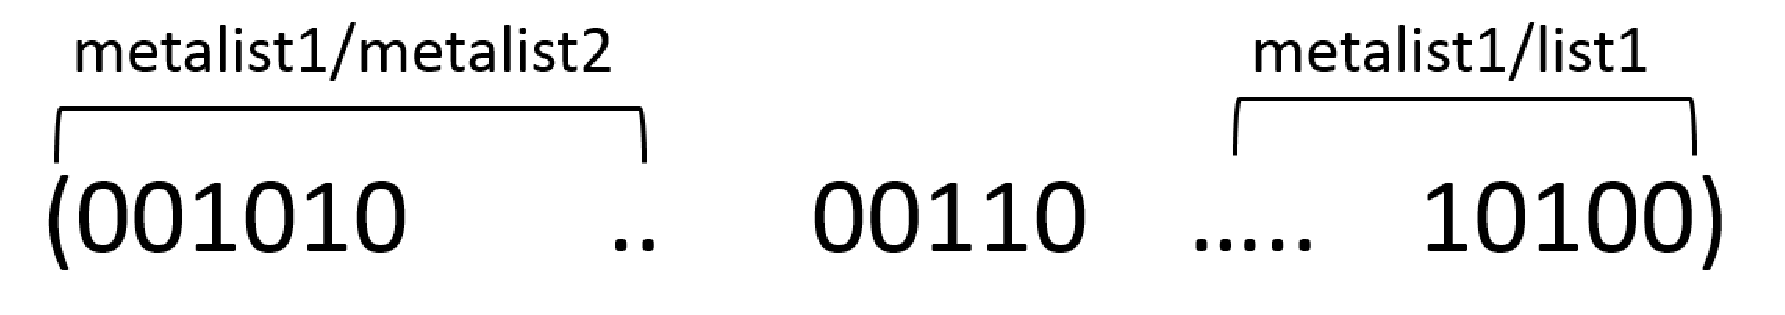
\epsfig{file=links_categorization.eps,height=1cm,width=6cm}
	      \end{center}
	    \end{slide}
	    \begin{slide}
	      \textbf{\textcolor{blue}{\large Semantic similarity}}\newline
	    We slack our universe by allowing links only between semantically similar URLs :
	    \begin{equation}
	    \max_{\left(G_{ij}\right)  \in \left\{0,1\right\}^{N\times N}\ G_{ij}=0 \ if \ CS(ij)\leq t}\left\{ \sum^{N}_{i=1} f\left(X_i\right)\times PR(X_i)\right\}
	    \end{equation}
	    where $CS(ij)$ is a semantic distance between the two linked pages $i$ and $j$.
	    \newline $CS(ij)$ can be defined very easily as the scalar product of the tf/idf vectors of the
	    product descriptions whose weight are defined by the well known formula :
	    \begin{equation}
	    w_{ik}=\frac{tf_{ik}\log\left( \frac{N}{n_k}\right)}{\sqrt{\sum_{k=1}^t}(tf_{ik})^2 \log\left(\frac{N}{n_k}\right)^2}
	    \end{equation}
	    \end{slide}
	    \begin{slide}
	    \slideheading{Same problem with an e-commerce flavor}
	  \begin{equation}
	  \sum_{i\in Keywords} SV\left( i\right)\times CTR\left(position\left(i\right)\right)\times PR\left(i\right)\times P\left(i\right)
	  \end{equation}
	  where $position\left(i\right)$ is the estimated position in search engine results coming from the modification of our new mesh,
	  \\\newline
	  $SV\left(i\right)$ is the search volume for the keywords $i$ estimated by the search engine.
	  \\\newline
	  and $CTR\left(i\right)$ is the click through rate for an URL at the position place in the search engine results.
	  \\\newline
	    \end{slide}
	    \begin{slide}
	    \slideheading{Prototyping example}
	    {\scriptsize{
	      $\left(X_i\right)$ ={'home','metalist1','metalist2','list1','list2','list3','list4','product1','product2',...,'product32'};
              $f\left(X_i\right)$=[   100,         80,         55,     40,     35,     25,     20,         4,         5,...,3          ];
	    }}
	\begin{center}
      \textbf{\large Results}
      \end{center}
      \begin{center}
      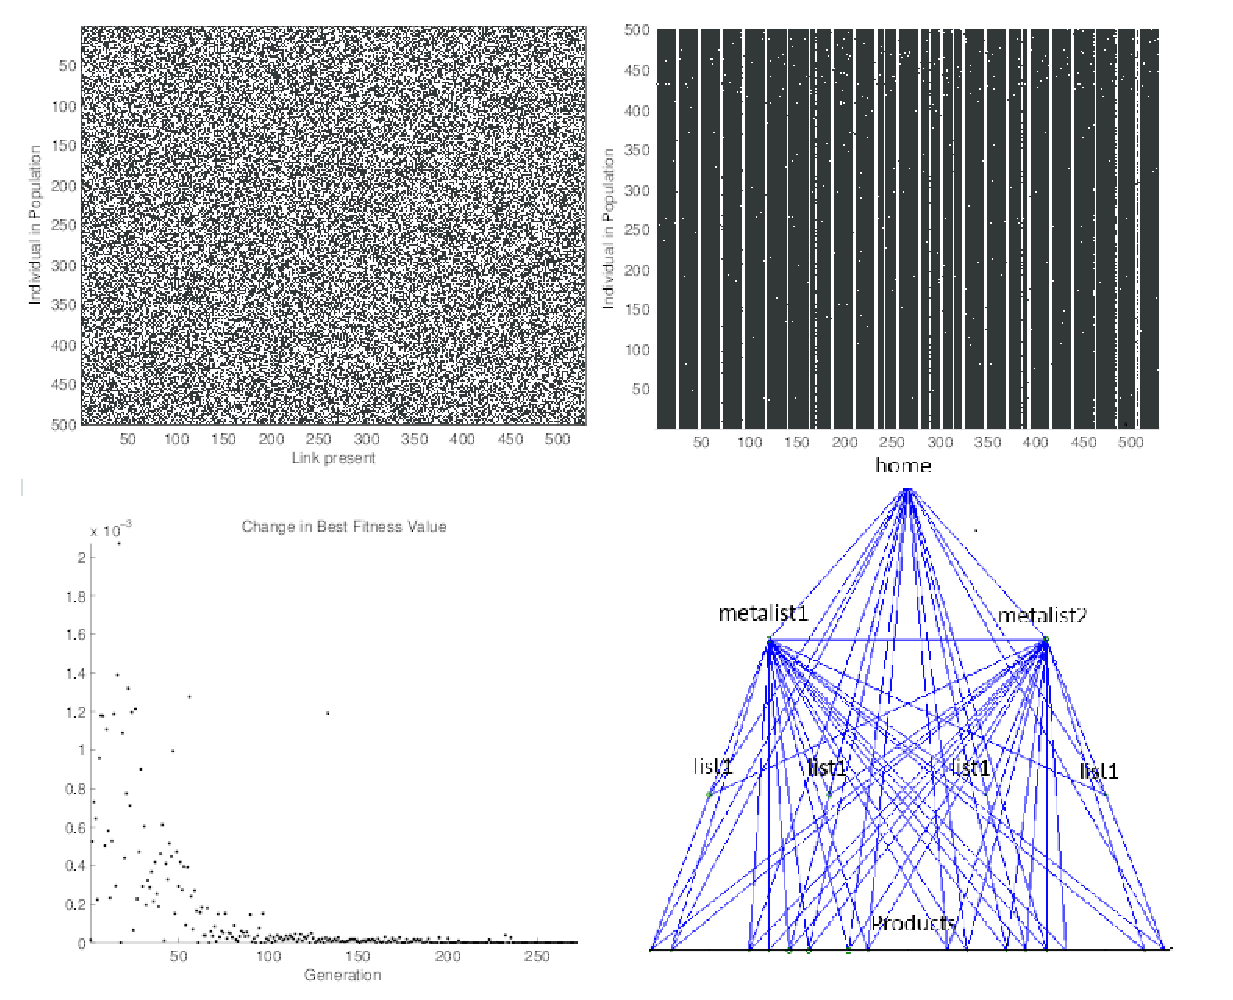
\epsfig{file=prototyping_example.eps,height=5.cm,width=5.cm}
      \end{center}
	    \end{slide}
	    \begin{slide}
	      \slideheading{Big data implementation : Neo4j and Spark GraphX}
	      \begin{center}
	      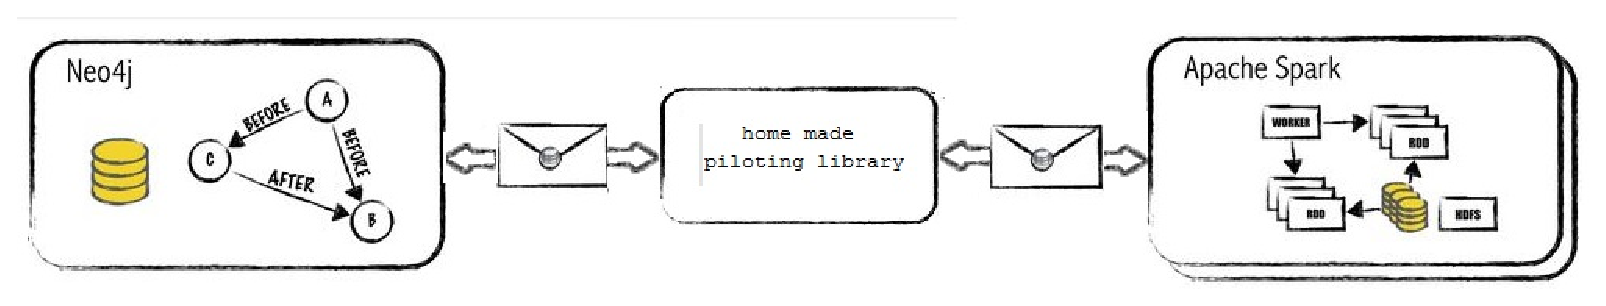
\epsfig{file=neo4j_maze_runner.eps,height=3.cm,width=12.cm}
	      \end{center}
	    \end{slide}
	    \begin{slide}
	     \slideheading{Video and paper link}
        	    \textbf{\textcolor{blue}{\normalsize http://sduprey.github.io/page\_rank\_optimization\_video.html}}\newline 
        	    \textbf{\textcolor{blue}{\normalsize http://sduprey.github.io/article\_sduprey\_iswag\_02\_06\_2015.pdf}}\newline 
       	            \textbf{\textcolor{blue}{\normalsize http://sduprey.github.io/PRESENTATION\_ISWAG.pdf}}\newline 
	    \end{slide} 
	    \end{document}